\appendix

\chapter{Requirements}\label{sec:requirements}

% TODO: Revisit requirements and add more details

\begin{table}[h!]
    \centering
    \begin{tabular}{|c|p{10cm}|c|}
    \hline
    \textbf{ID}  & \textbf{Requirement}  & \textbf{Priority} \\ \hline
    1.1  & The system must be accessible on all modern desktop and mobile-based browsers.       & Must Have \\ \hline
    1.2  & The system must be accessible from any location by using an internet connection.     & Must Have \\ \hline
    1.3  & The system must store the data in a secure manner, ensuring that only the patient and the doctor can access the data. & Must Have \\ \hline
    1.4  & When shared with the doctor via a link, the system must load within 3 to 5 seconds when accessed via a desktop browser. & Should Have \\ \hline
    1.5  & When shared with the doctor via a link, the system should secure the data with a unique token or PIN that expires after the specified time frame. & Could Have \\ \hline
    1.6  & The system could be accessible on all modern mobile devices via a mobile application. & Could Have \\ \hline
    \end{tabular}
    \caption{Non-functional Requirements}
\end{table}
    
\begin{table}[h!]
    \centering
    \begin{tabular}{|c|p{10cm}|c|}
    \hline
    \textbf{ID}  & \textbf{Requirement}  & \textbf{Priority} \\ \hline
    2.1  & The system must provide a secure login mechanism for patients by using a combination of login and password. & Must Have \\ \hline
    2.2 & The database must store the user credentials in a secure manner. & Must Have \\ \hline
    2.3 & The system could provide an option for multi factor authentication. & Could Have \\ \hline
    2.4 & The system could provide an option for password recovery. & Could Have \\ \hline
    2.5  & If used on mobile, the system could allow the patient to use biometric authentication for logging in. & Should Have \\ \hline
    \end{tabular}
    \caption{Login Requirements}
\end{table}

\begin{table}[h!]
    \centering
    \begin{tabular}{|c|p{10cm}|c|}
    \hline
    \textbf{ID}  & \textbf{Requirement}  & \textbf{Priority} \\ \hline
    3.1  & The system must allow patients to upload their own medical records in a variety of formats (PDF, DOC, etc). & Must Have \\ \hline
    3.2 & The system should allow to upload files/documents for other types of records (vaccine certificates, etc). & Should Have \\ \hline
    3.2  & The system must allow the patient to specify and categorise the type of document they are uploading (lab test, doctor consultation, etc). & Must Have \\ \hline
    3.3 & The system must allow the patient to add a description of the document they are uploading. & Must Have \\ \hline
    3.4 & The system should allow the patient to add a date for the document they are uploading. & Should Have \\ \hline
    3.5 & The system should allow the patient to add a location for the document they are uploading. & Should Have \\ \hline
    3.6 & The system should allow the patient to add the doctor name for the document they are uploading. & Should Have \\ \hline
    3.7 & The system should allow the patient to sort and filter the documents based on the type of document, date, location, and doctor name. & Should Have \\ \hline
    3.8 & If used on mobile, the system should allow the patient to take a picture of the document and upload it. & Could Have \\ \hline
    \end{tabular}
    \caption{Document Upload Requirements}
\end{table}

\begin{table}[h!]
    \centering
    \begin{tabular}{|c|p{10cm}|c|}
    \hline
    \textbf{ID}  & \textbf{Requirement}  & \textbf{Priority} \\ \hline
    4.1  & The system must allow the patient to generate a shareable link to provide access to their medical records. & Must Have \\ \hline
    4.2  & When creating the shareable link, the system must allow the patient to set an expiration date for the link. & Must Have \\ \hline
    4.3  & When creating the shareable link, the system should allow the patient to set an access password for the link. & Should Have \\ \hline
    4.4  & When creating the shareable link, the system should allow the patient to select which records to share with the doctor. & Should Have \\ \hline
    \end{tabular}
    \caption{Patient Shareable Link Requirements}
\end{table}

\begin{table}[h!]
    \centering
    \begin{tabular}{|c|p{10cm}|c|}
    \hline
    \textbf{ID}  & \textbf{Requirement}  & \textbf{Priority} \\ \hline
    5.1  & The patient personal cabinet must provide an overview of the patient's history through 3 main sections: personal information, lab tests, and doctor consultations. & Must Have \\ \hline
    5.2  & The system must display the patient's history in a chronological order in the form of a timeline. & Must Have \\ \hline
    5.3 & The system must have a dashboard view which displays an overview of the most recent information added to the system (latest lab tests, doctor consultations, vaccinations etc). & Must Have \\ \hline
    5.4  & The system must allow patients to add their own personal information, such as name or date of birth. & Must Have \\ \hline
    5.5  & The system must allow the patient to add their own allergies. & Must Have \\ \hline
    5.6  & The system must allow the patient to add their own vaccinations. & Must Have \\ \hline
    5.7  & When viewing doctor consultations, the system should divide them into categories based on the domain of the doctor (cardiology, neurology, etc). & Should Have \\ \hline
    5.8  & The system should allow the patient to enter vitals information, such as height, weight, blood pressure, etc. & Should Have \\ \hline
    5.9  & The system should display the information in both a list or grid view. & Should Have \\ \hline
    5.10  & When multiple vital entries are made, the system could display a historical graph of the patient's vitals. & Could Have \\ \hline
    5.11 & The system could allow the patient to switch between viewing the lab tests in the document format or in a tabular, numerical format. & Could Have \\ \hline
    \end{tabular}
    \caption{Patient Personal Cabinet Requirements}
\end{table}

\begin{table}[h!]
    \centering
    \begin{tabular}{|c|p{10cm}|c|}
    \hline
    \textbf{ID}  & \textbf{Requirement}  & \textbf{Priority} \\ \hline
    6.1  & The system must provide an overview of the patient history through 3 main sections: personal information, lab tests, and doctor consultations. & Must Have \\ \hline
    6.2  & When shared with the doctor, the system must allow the doctor to only view the patient's history, not edit it. & Must Have \\ \hline
    6.3  & The system must allow the doctor to view blood tests in a graphical format. & Must Have \\ \hline
    6.4  & The system must allow the doctor to view blood tests in a numerical, tabular format. & Must Have \\ \hline
    6.5  & The system must allow the doctor to view the patient's history in a chronological order. & Must Have \\ \hline
    6.6  & The system must display the doctor consultation and every lab test, except for blood tests, in a free text or document format. & Must Have \\ \hline
    6.7  & When viewing blood test results, the system should show the source document of the blood test value. & Should Have \\ \hline
    6.8  & For blood test results, the system should display the normal range values for each test. & Should Have \\ \hline
    \end{tabular}
    \caption{Shared Patient Information Requirements (Doctor View)}
\end{table}

\begin{table}[h!]
    \centering
    \begin{tabular}{|c|p{10cm}|c|}
    \hline
    \textbf{ID}  & \textbf{Requirement}  & \textbf{Priority} \\ \hline
    7.1  & The system must allow patients to enter their current medication including details such as the name of the drug, dosage, frequency and start/end date. & Must Have \\ \hline
    7.2 & The system must allow patients to add new medication to their list. & Must Have \\ \hline
    7.3 & When adding medication, the system should have 2 options: add a simplified version of the medication or add a detailed version of the medication. & Should Have \\ \hline
    7.4 & When choosing the simplified version, the system should allow the patient to just add the name, dosage and duration of the medication. & Should Have \\ \hline
    7.5 & When choosing the detailed version, the system should allow the patient to add the name, dosage, frequency, start/end date, and the reason for taking the medication. & Should Have \\ \hline
    7.6  & The system should allow patients to add their past medication & Should Have \\ \hline
    7.7  & The system should allow patients to set medication reminders. & Should Have \\ \hline
    7.8 & After entering the medication, the system could allow the patient to track the medication intake. & Could Have \\ \hline

    \end{tabular}
    \caption{Patient Medication Requirements}
\end{table}

\chapter{Wireframes}\label{sec:wireframes}

\begin{figure}[ht]
    \centering
    \subfloat[Desktop version]{%
        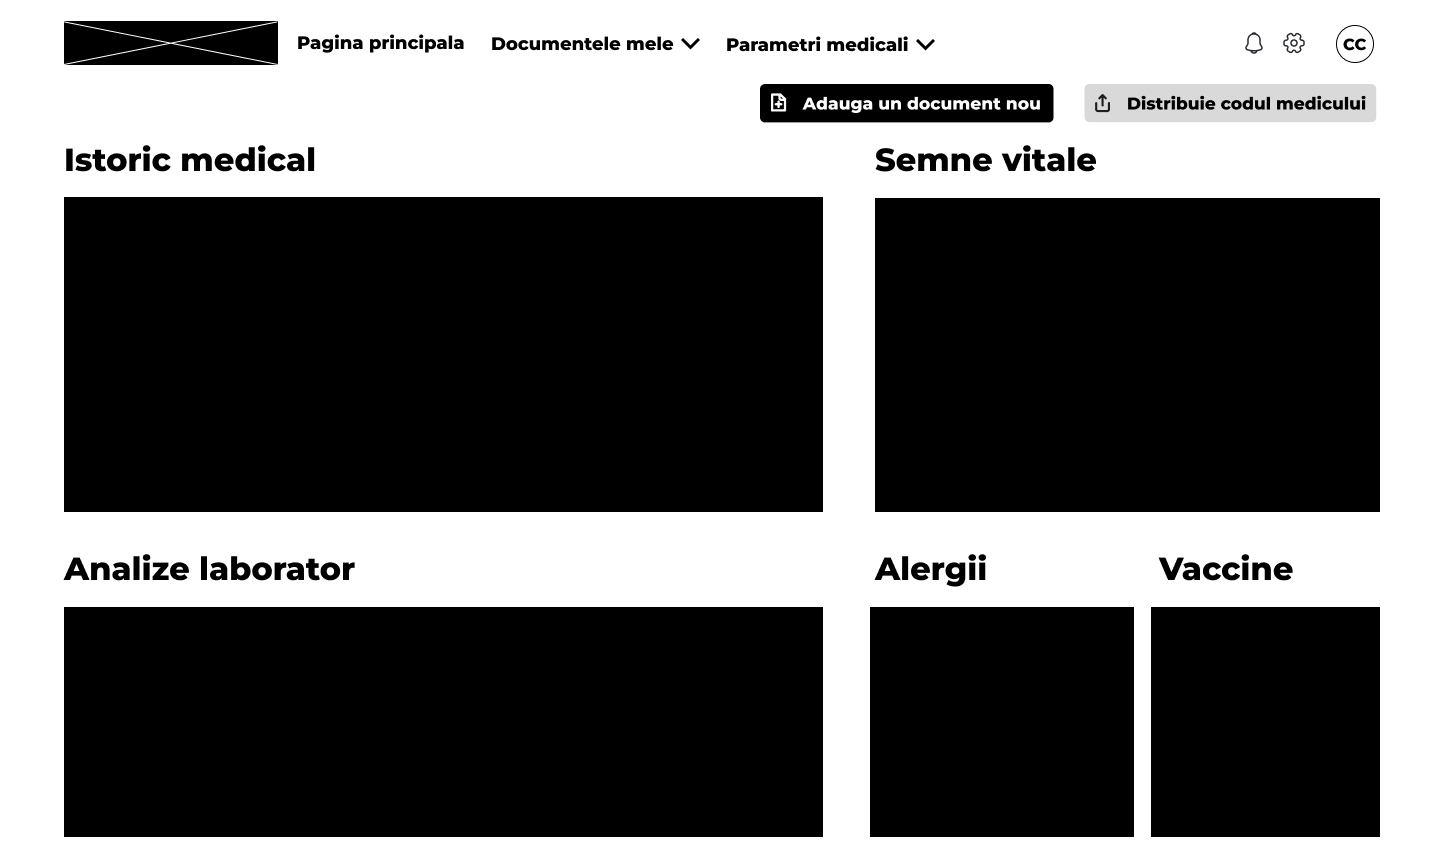
\includegraphics[width=0.75\textwidth]{wireframes/Desktop_dashboard.png}%
    }
    \hspace{0.05\textwidth}
    \subfloat[Mobile version]{%
        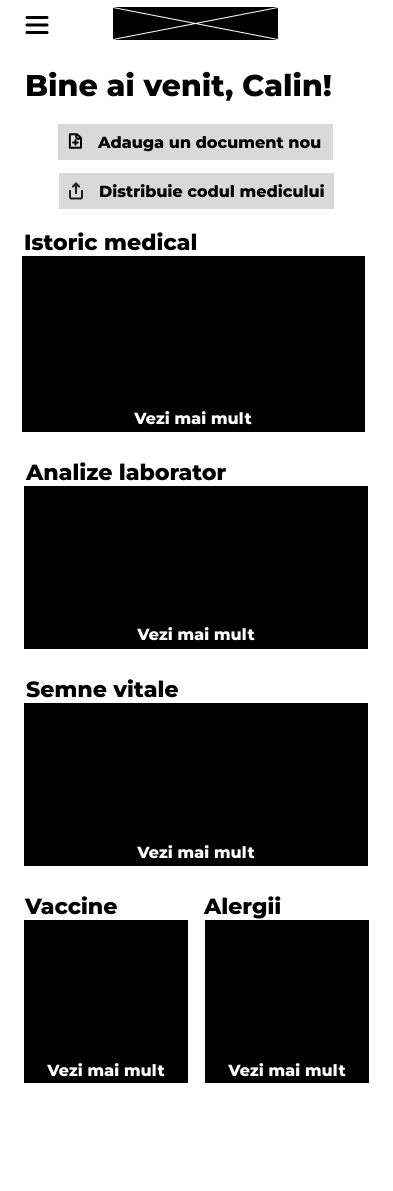
\includegraphics[scale=0.25]{wireframes/Mobile_dashboard.png}%
    }
    \caption{Desktop and Mobile version of the Dashboard screen}
\end{figure}

\begin{figure}[ht]
    \centering
    \subfloat[Desktop version]{%
        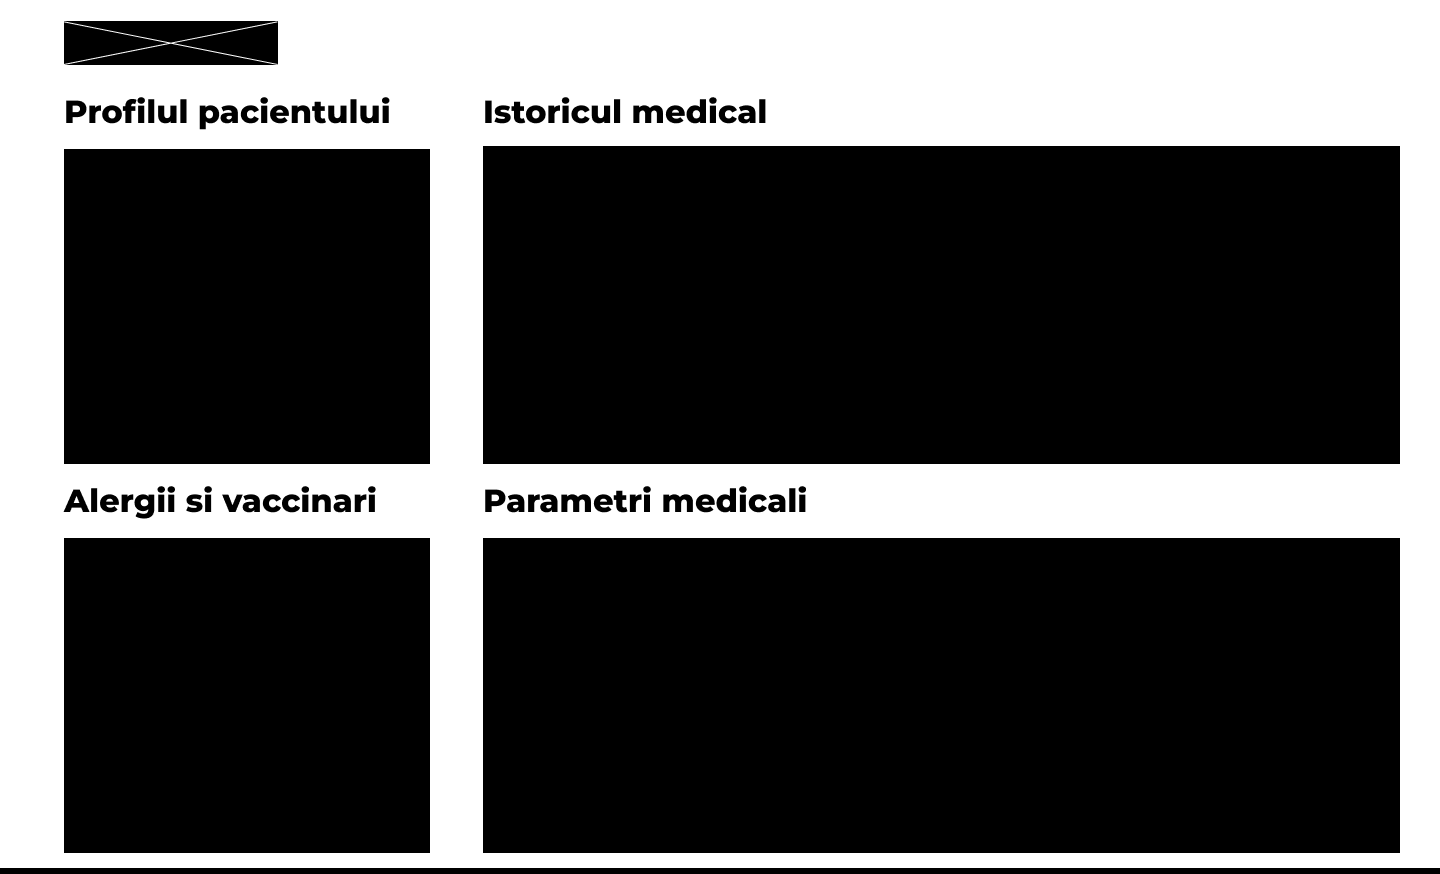
\includegraphics[width=0.75\textwidth]{wireframes/Desktop_doctorView.png}%
    }
    \hspace{0.05\textwidth}
    \subfloat[Mobile version]{%
        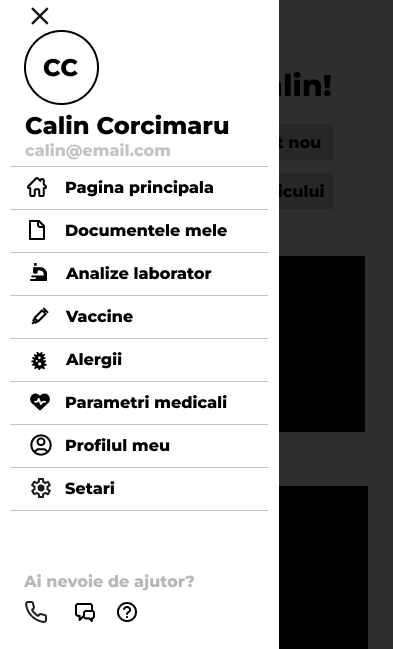
\includegraphics[scale=0.3]{wireframes/Mobile_dashboardMenu.png}%
    }
    \caption{Desktop and Mobile version of the Doctor View screen}
\end{figure}

\begin{figure}[ht]
    \centering
    \subfloat[Desktop version]{%
        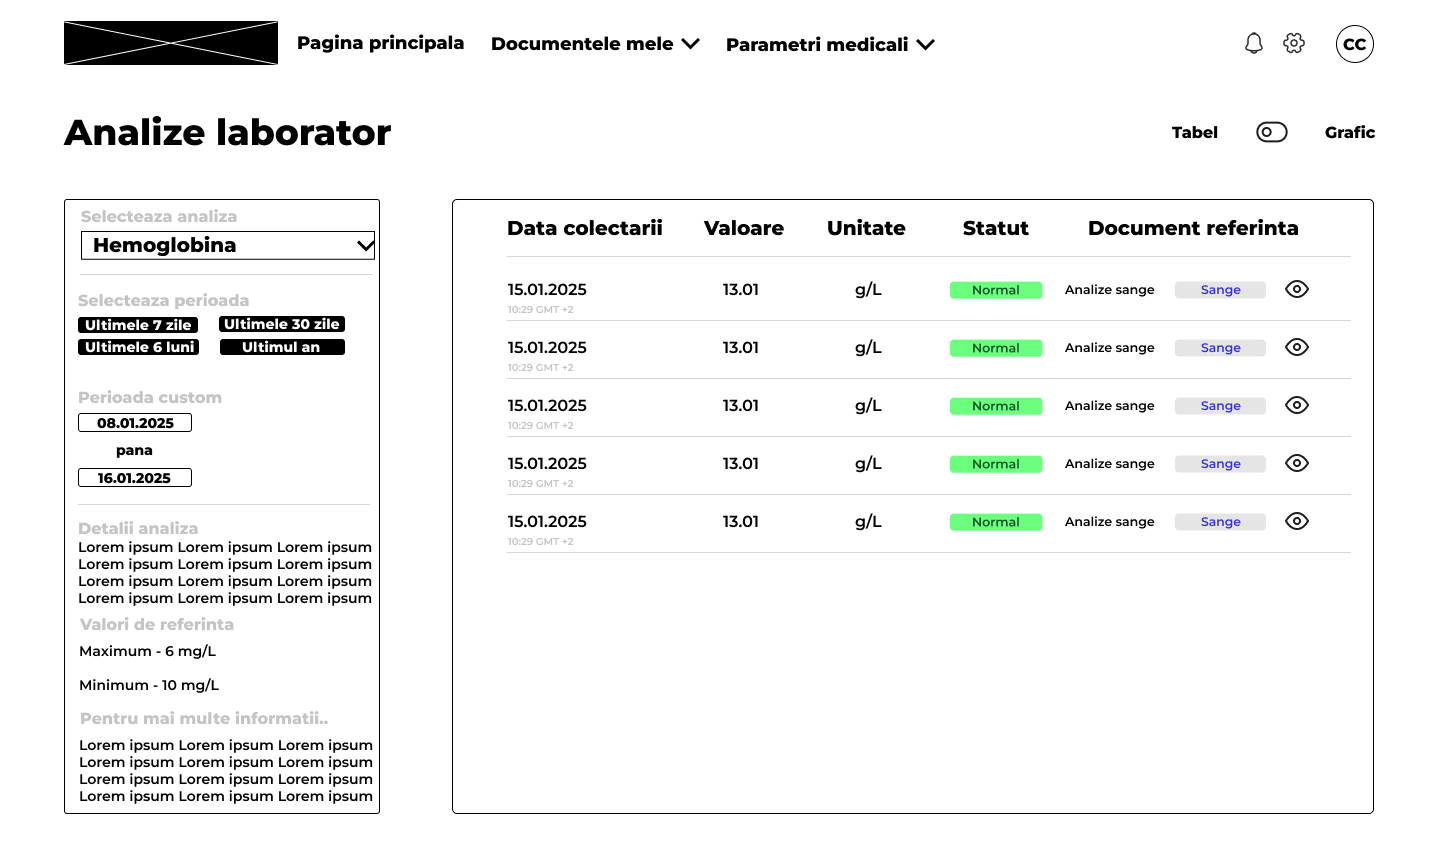
\includegraphics[width=0.75\textwidth]{wireframes/Desktop_labTest.png}%
    }
    \hspace{0.05\textwidth}
    \subfloat[Mobile version]{%
        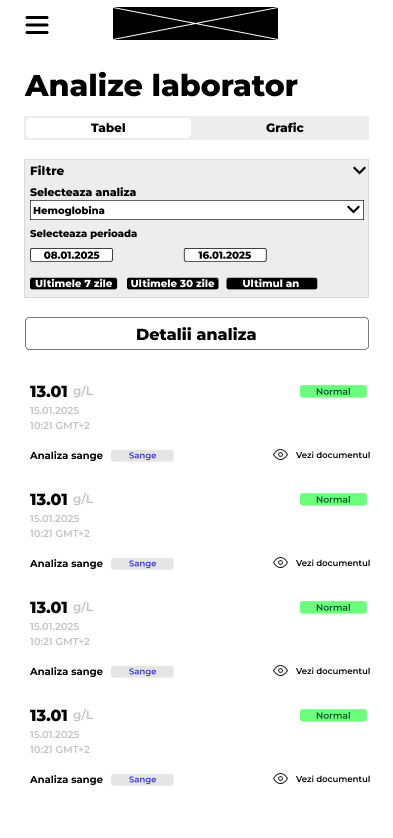
\includegraphics[scale=0.3]{wireframes/Mobile_labTest.png}%
    }
    \caption{Desktop and Mobile version of the Lab Test screen}
\end{figure}

\begin{figure}[ht]
    \centering
    \subfloat[Desktop version]{%
        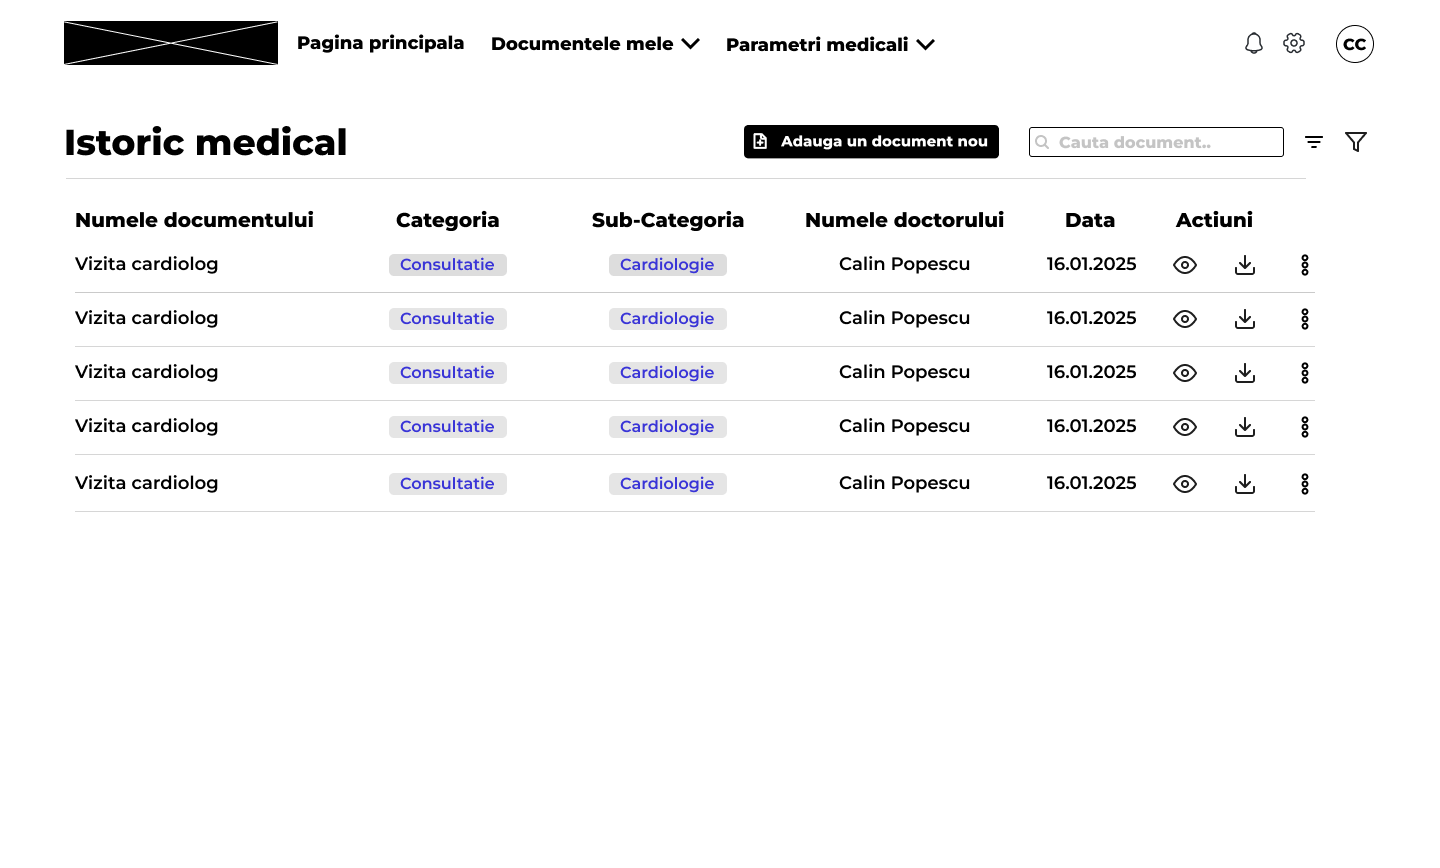
\includegraphics[width=0.75\textwidth]{wireframes/Desktop_medHistory.png}%
    }
    \hspace{0.05\textwidth}
    \subfloat[Mobile version]{%
        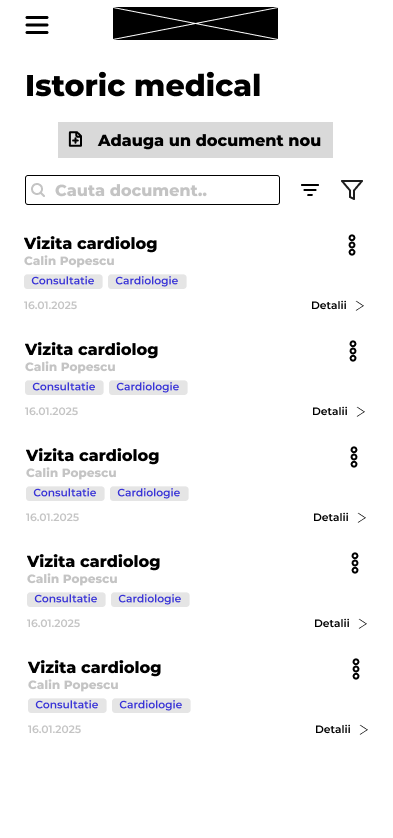
\includegraphics[scale=0.3]{wireframes/Mobile_medHistory.png}%
    }
    \caption{Desktop and Mobile version of the Medical History screen}
\end{figure}

\begin{figure}[ht]
    \centering
    \subfloat[Desktop version]{%
        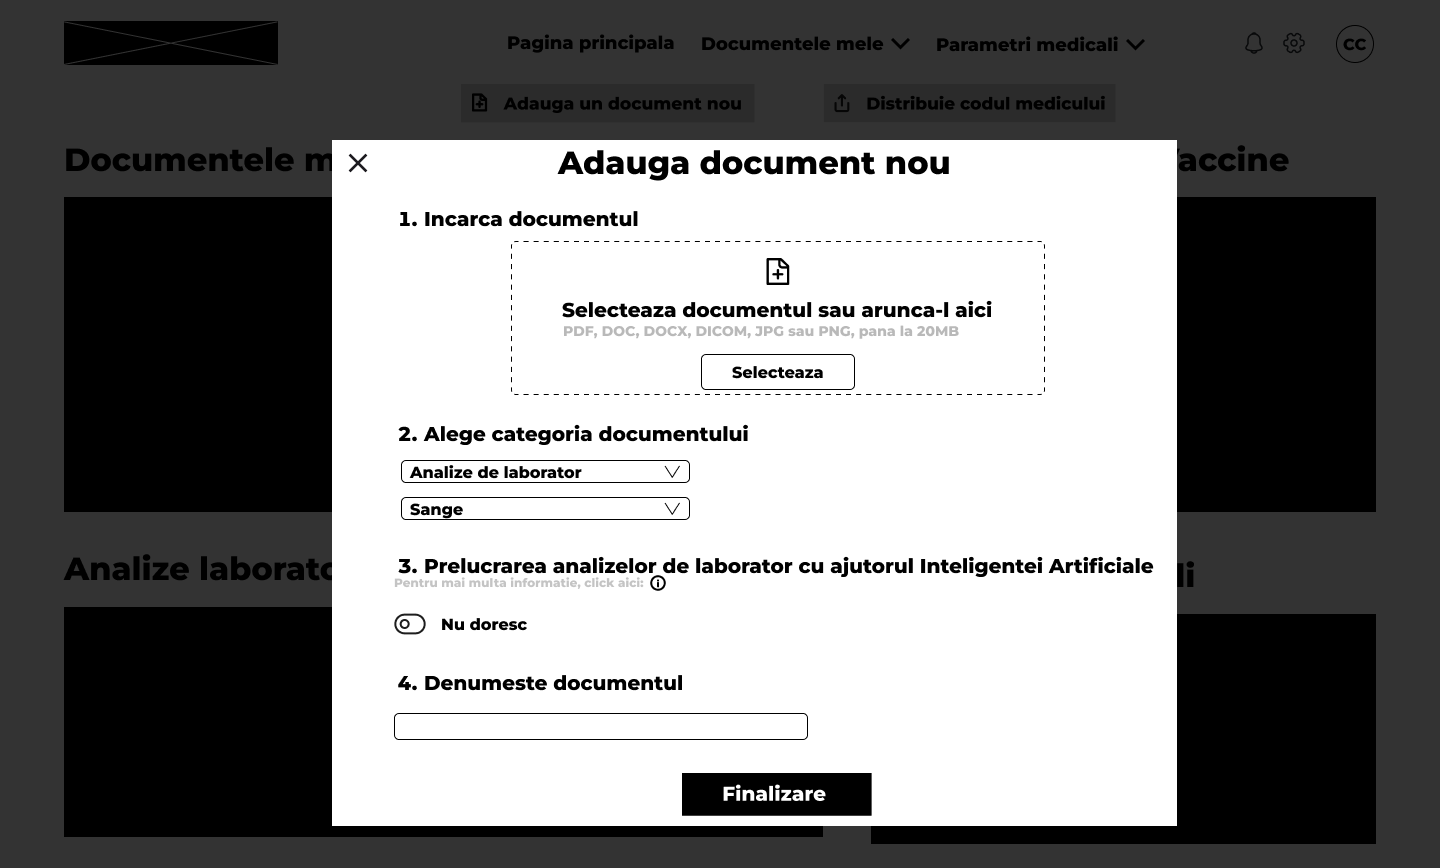
\includegraphics[width=0.70\textwidth]{wireframes/Desktop_newDoc.png}%
    }
    \hspace{0.05\textwidth}
    \subfloat[Mobile version]{%
        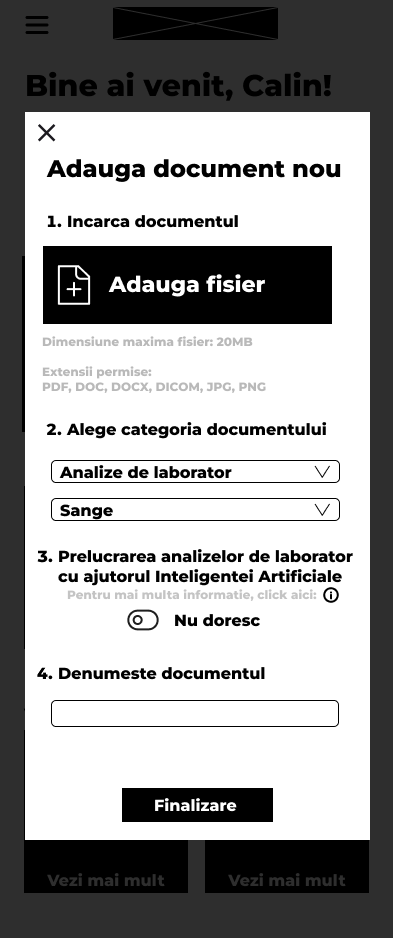
\includegraphics[scale=0.3]{wireframes/Mobile_newDoc.png}%
    }
    \caption{Desktop and Mobile version of the New Document screen}\label{fig:newDoc_wireframe}
\end{figure}

\begin{figure}[ht]
    \centering
    \subfloat[Desktop version]{%
        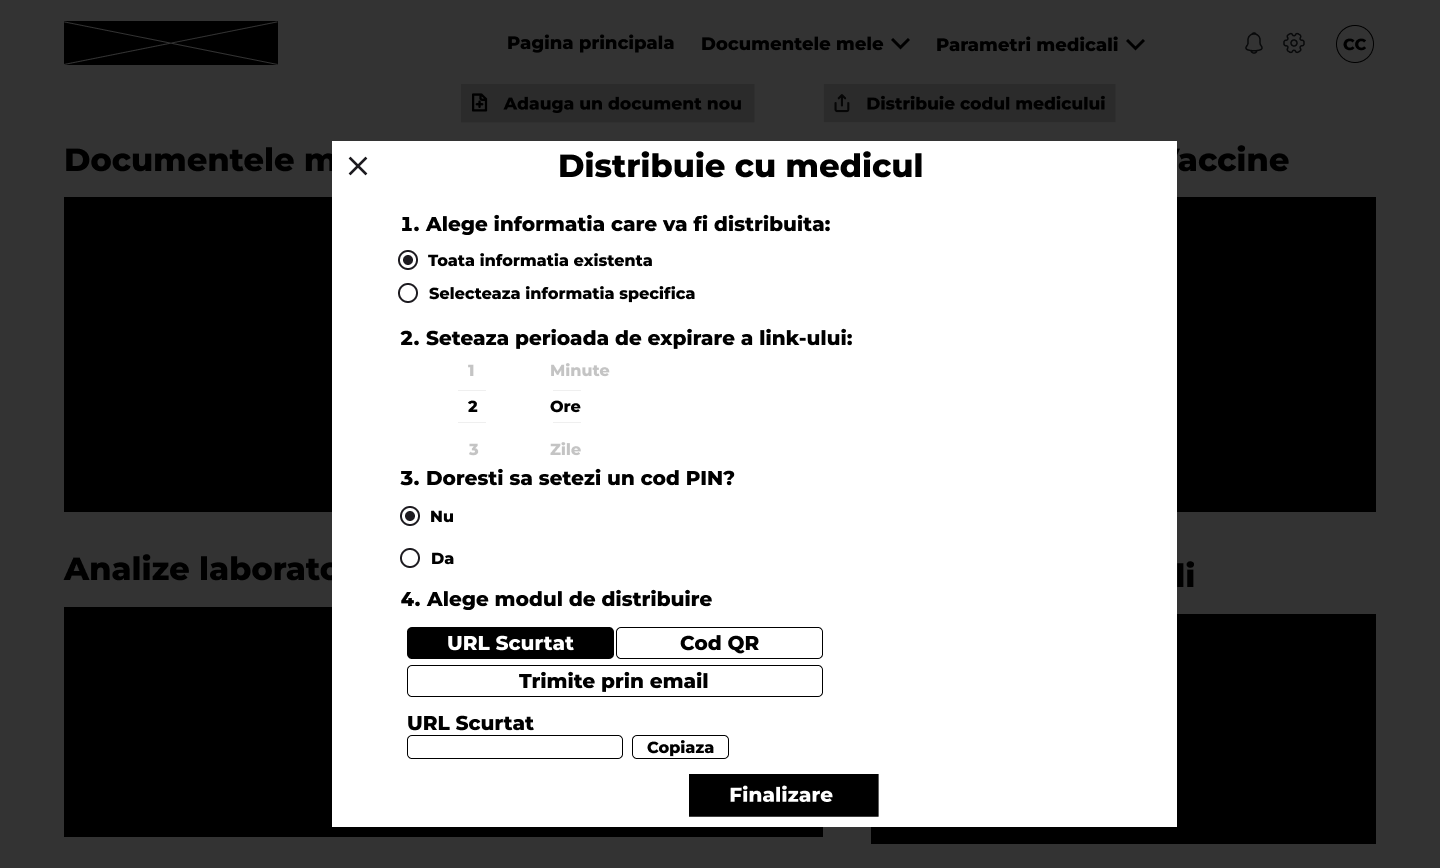
\includegraphics[width=0.75\textwidth]{wireframes/Desktop_shareDoctor.png}%
    }
    \hspace{0.05\textwidth}
    \subfloat[Mobile version]{%
        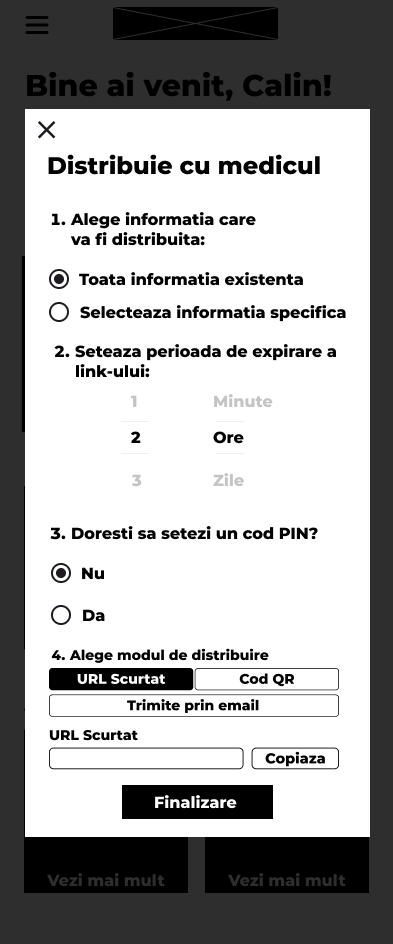
\includegraphics[scale=0.3]{wireframes/Mobile_shareDoctor.png}%
    }
    \caption{Desktop and Mobile version of the Share Doctor screen}
\end{figure}

\begin{figure}[ht]
    \centering
    \subfloat[Desktop version]{%
        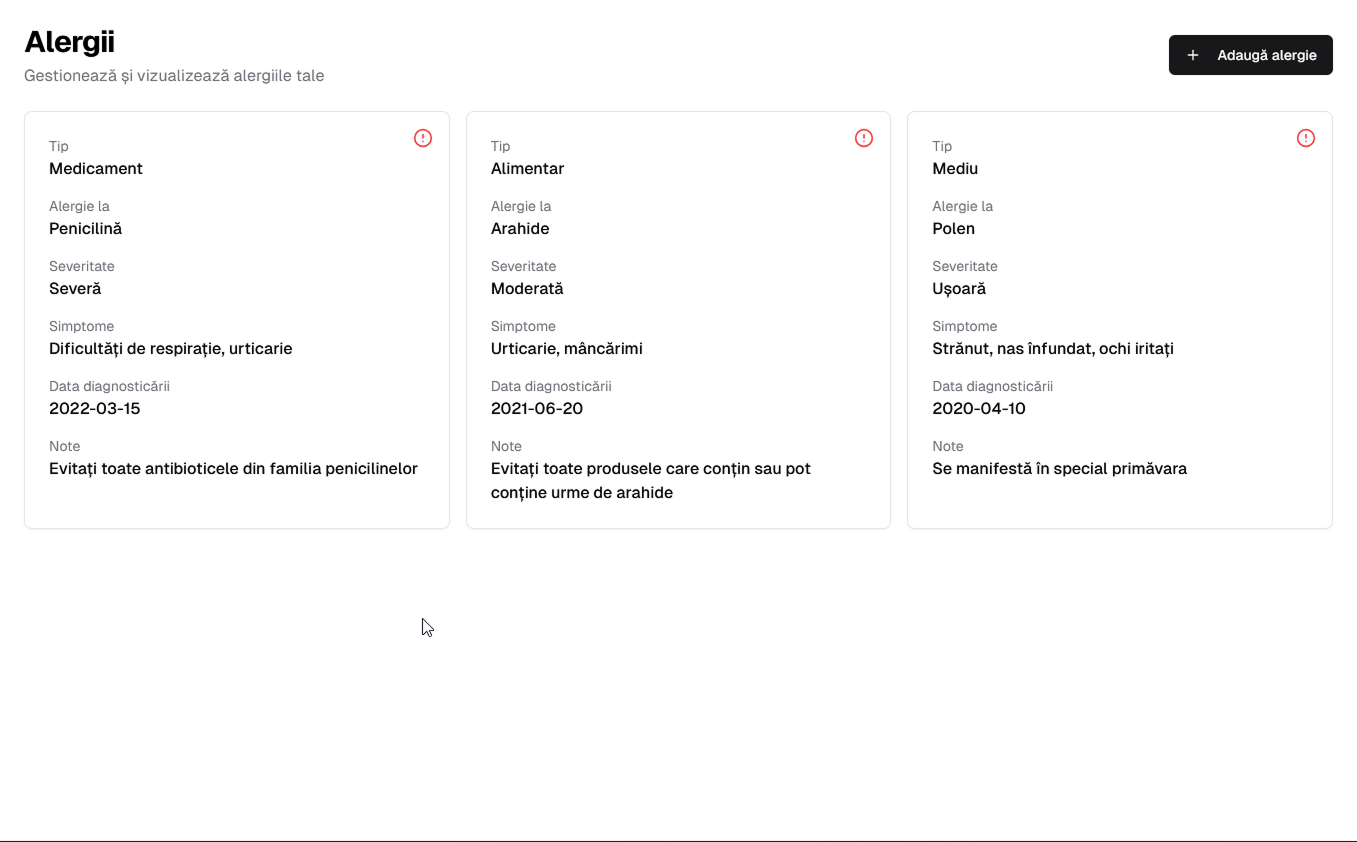
\includegraphics[width=0.75\textwidth]{wireframes/AI-allergies-desktop.png}%
    }
    \hspace{0.05\textwidth}
    \subfloat[Mobile version]{%
        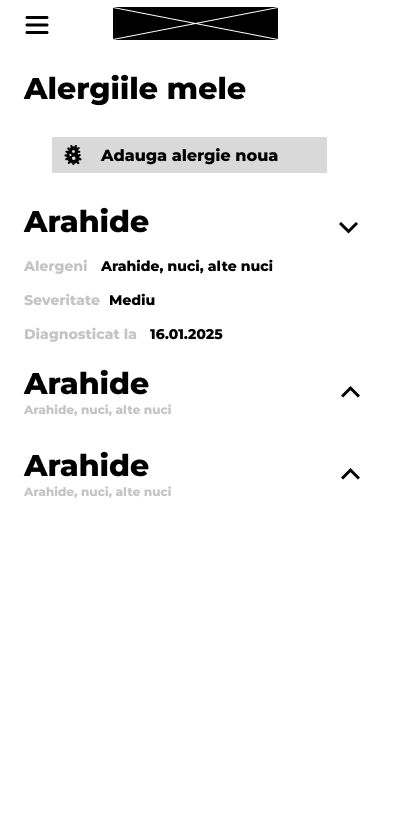
\includegraphics[scale=0.3]{wireframes/Mobile_allergies.png}%
    }
    \caption{Desktop and Mobile version of the Allergies screen}
\end{figure}

\begin{figure}[ht]
    \centering
    
\includegraphics[width=0.3\textwidth]{wireframes/Mobile_vaccines.png}
    \caption{Mobile version of the Vaccines screen}
\end{figure}